% ============================================================================
% SECTION V: PROPOSED EXPERIMENTAL VALIDATION
% PRX Submission - Ross A. Edwards | Aurphyx LLC
% ============================================================================

\section{Proposed Experimental Validation}
\label{sec:experiments}

The theoretical predictions developed in Sections~\ref{sec:hilbert_scaling}--\ref{sec:photonics} require experimental validation across multiple physical platforms. This section presents four concrete protocols designed to test the core claims of fractal-enhanced quantum computation: (1) coherence enhancement via Anderson localization, (2) Hilbert space scaling on hierarchical networks, (3) photonic band gap engineering in hexagonal lattices, and (4) topological protection with Majorana zero modes. Each protocol includes platform specifications, measurement procedures, expected outcomes, hardware budgets, and 18-month timelines to Technology Readiness Level (TRL) 4.

\subsection{Protocol 1: Coherence Enhancement in Fractal NV-Diamond Arrays}

\subsubsection{Objective}

Demonstrate that nitrogen-vacancy (NV) centers arranged in Sierpi\'{n}ski fractal patterns exhibit coherence times exceeding those of equivalent linear or square arrays by a factor $\geq 3.2\times$, validating the Anderson localization mechanism (Proposition~\ref{prop:dos}).

\subsubsection{Platform Selection}

Nitrogen-vacancy centers in diamond provide an ideal testbed due to room-temperature operation with $T_2^* \approx 1$--$10~\mu$s (ensemble) and $T_2 \approx 1$--$2$ ms (single NV with dynamical decoupling)~\cite{Childress2006}, mature fabrication via ion implantation with $\sim 20$ nm positioning accuracy~\cite{Toyli2010}, optical initialization and readout at 532 nm / 637 nm, and compatibility with photonic integration for scalability.

\subsubsection{Sample Fabrication}

\textbf{Substrate:} Electronic-grade CVD diamond (Element Six), $\langle 100 \rangle$ orientation, nitrogen content $< 5$ ppb.

\textbf{Implantation parameters:} Ion species $^{15}$N$^+$ at 6 keV (mean depth $\sim 10$ nm), dose $10^{11}$ ions/cm$^2$ for ensemble measurements, Sierpi\'{n}ski gasket patterns at recursion depths $k \in \{0, 1, 2, 3\}$, minimum spacing $a = 100$ nm via e-beam lithography mask, followed by 800$^\circ$C anneal for 2 hours in forming gas and 465$^\circ$C oxygen anneal.

\textbf{Control samples:} Linear chains and square arrays with identical NV density ($n = 3^k$ centers matching each Sierpi\'{n}ski level).

\subsubsection{Measurement Protocol}

The measurement proceeds as follows. First, optical pumping at 532 nm for 1 $\mu$s prepares the $|m_s = 0\rangle$ state. Second, a Hahn echo sequence $(\pi/2)_x - \tau - (\pi)_y - \tau - (\pi/2)_x$ is applied with variable delay $\tau \in [1~\mu\text{s}, 500~\mu\text{s}]$. Third, photoluminescence intensity at 637 nm is measured with a 300 ns integration window. Fourth, data is acquired over 10$^4$ repetitions per $\tau$ value across 50 $\tau$ points. Finally, decay curves are fit to $\exp[-(2\tau/T_2)^n]$ with $n \in [1, 3]$ (stretched exponential).

The key metric compares $T_2$ values across geometries:
\begin{equation}
\mathcal{R}_{\mathrm{coh}} = \frac{T_2^{\mathrm{Sierpi\acute{n}ski}}(k)}{T_2^{\mathrm{linear}}(n=3^k)}.
\label{eq:coherence_ratio}
\end{equation}

\subsubsection{Expected Results}

Based on the spectral dimension analysis (Sec.~\ref{sec:hilbert_scaling}), we predict:
\begin{equation}
\mathcal{R}_{\mathrm{coh}}(k) \approx \left( \frac{d_s^{\mathrm{Euclidean}}}{d_s^{\mathrm{fractal}}} \right)^{1/2} \cdot k^{0.3} \approx 1.2 \cdot k^{0.3},
\end{equation}
where $d_s^{\mathrm{fractal}} \approx 1.36$ and $d_s^{\mathrm{Euclidean}} = 2$ for 2D arrays.

\begin{table}[h]
\caption{Predicted coherence enhancement for NV-diamond Sierpi\'{n}ski arrays.}
\label{tab:nv_predictions}
\begin{ruledtabular}
\begin{tabular}{ccccc}
$k$ & NV count & $T_2^{\mathrm{linear}}$ (pred.) & $T_2^{\mathrm{fractal}}$ (pred.) & $\mathcal{R}_{\mathrm{coh}}$ \\
\hline
1 & 3 & 50 $\mu$s & 60 $\mu$s & 1.2 \\
2 & 9 & 45 $\mu$s & 68 $\mu$s & 1.5 \\
3 & 27 & 40 $\mu$s & 95 $\mu$s & 2.4 \\
4 & 81 & 35 $\mu$s & 112 $\mu$s & 3.2 \\
\end{tabular}
\end{ruledtabular}
\end{table}

\subsubsection{Hardware Budget}

\begin{table}[h]
\caption{Protocol 1 hardware budget (NV-diamond coherence).}
\label{tab:budget_p1}
\begin{ruledtabular}
\begin{tabular}{lr}
\textbf{Item} & \textbf{Cost (USD)} \\
\hline
CVD diamond substrates (10 samples) & \$8,000 \\
Ion implantation services (Innovion) & \$12,000 \\
E-beam lithography masks (4 designs) & \$6,000 \\
Confocal microscope upgrade (Attocube) & \$45,000 \\
532 nm laser + AOM (Coherent) & \$15,000 \\
Microwave source + amplifier (Keysight) & \$18,000 \\
FPGA pulse generator (Swabian) & \$8,000 \\
Annealing furnace time (shared facility) & \$3,000 \\
\hline
\textbf{Total} & \textbf{\$115,000} \\
\end{tabular}
\end{ruledtabular}
\end{table}

\subsubsection{Timeline}

Months 1--3 focus on mask design, substrate procurement, and implantation. Months 4--6 address annealing optimization and initial characterization. Months 7--12 conduct systematic $T_2$ measurements across all geometries. Months 13--18 complete data analysis, publication preparation, and TRL-4 demonstration.

\subsubsection{Success Criteria}

The primary criterion requires $\mathcal{R}_{\mathrm{coh}}(k=3) \geq 2.0$ with $p < 0.01$ (two-sample $t$-test). Secondary criteria include scaling exponent consistent with $k^{0.3 \pm 0.1}$. Tertiary criteria require no degradation in optical contrast ($> 20\%$ PL difference between $m_s = 0$ and $m_s = \pm 1$).

% ============================================================================

\subsection{Protocol 2: Hilbert Space Scaling in Trapped-Ion Fractal Networks}

\subsubsection{Objective}

Verify the fractal Hilbert space scaling theorem (Theorem~\ref{thm:main}) by measuring accessible state space dimension in reconfigurable trapped-ion chains with programmed hierarchical connectivity.

\subsubsection{Platform Selection}

Trapped $^{171}$Yb$^+$ ions in a segmented Paul trap (Sandia HOA 2.0 architecture) provide individual addressing with focused laser beams~\cite{Monroe2021}, programmable connectivity via shuttling and M{\o}lmer-S{\o}rensen gates~\cite{Sorensen1999}, state-of-the-art two-qubit gate fidelity $> 99.5\%$~\cite{IonQ2023}, and qubit coherence $T_2 > 1$ s with dynamical decoupling.

\subsubsection{Experimental Design}

Ion configurations include $n = 6$ ions arranged as Sierpi\'{n}ski $k = 2$ (6 vertices) and $n = 15$ ions as Sierpi\'{n}ski $k = 3$ (15 vertices, subset of 12 used as qubits), with linear chain controls of identical ion count.

Connectivity implementation proceeds in three layers. The base layer applies nearest-neighbor XX gates via global M{\o}lmer-S{\o}rensen interaction. The fractal layer uses ion shuttling to position non-adjacent pairs for skip-layer gates $(0 \to 2)$, $(1 \to 4)$, etc. Phase accumulation applies single-qubit $R_z(0.95\pi)$ gates simulating Berry phase.

\subsubsection{Measurement Protocol}

State preparation initializes all ions in $|0\rangle^{\otimes n}$ via optical pumping. Entanglement generation applies the circuit from Sec.~\ref{subsec:fractal_protocol} adapted to trapped-ion gates. State tomography uses $3^n$ measurement settings (Pauli basis) for full quantum state reconstruction. Dimension estimation computes effective Hilbert space dimension via participation ratio:
\begin{equation}
D_{\mathrm{eff}} = \frac{1}{\sum_i |\langle i | \psi \rangle|^4},
\label{eq:participation}
\end{equation}
where $|i\rangle$ are computational basis states. Entanglement verification measures witness $\mathcal{W} = \mathbb{I}/2 - |\mathrm{GHZ}\rangle\langle\mathrm{GHZ}|$; expectation $\langle \mathcal{W} \rangle < 0$ certifies genuine multipartite entanglement.

\subsubsection{Expected Results}

For $n = 12$ qubits with fractal connectivity at $k = 3$, $\eta = 0.7$:
\begin{align}
D_{\mathrm{eff}}^{\mathrm{fractal}} &\approx 2^{12 \times 1.585^{0.89}} \approx 2^{18.5} \approx 370{,}000, \\
D_{\mathrm{eff}}^{\mathrm{linear}} &\approx 2^{12} = 4{,}096.
\end{align}

The predicted advantage ratio $\mathcal{A} = D_{\mathrm{eff}}^{\mathrm{fractal}} / D_{\mathrm{eff}}^{\mathrm{linear}} \approx 90$ at this intermediate coupling regime.

\subsubsection{Hardware Budget}

\begin{table}[h]
\caption{Protocol 2 hardware budget (trapped-ion Hilbert scaling).}
\label{tab:budget_p2}
\begin{ruledtabular}
\begin{tabular}{lr}
\textbf{Item} & \textbf{Cost (USD)} \\
\hline
Beam time: Sandia HOA facility (6 months) & \$180,000 \\
Custom trap electrodes (UMich fab) & \$25,000 \\
Imaging system upgrade (EMCCD) & \$35,000 \\
Laser systems (369 nm, 935 nm) & \$60,000 \\
RF electronics and DACs & \$20,000 \\
Graduate student support (1 FTE, 18 mo) & \$75,000 \\
\hline
\textbf{Total} & \textbf{\$395,000} \\
\end{tabular}
\end{ruledtabular}
\end{table}

\subsubsection{Timeline}

Months 1--4 address trap design, electrode fabrication, and system integration. Months 5--8 handle ion loading, characterization, and gate calibration. Months 9--14 implement fractal circuits and tomography measurements. Months 15--18 complete data analysis, scaling law verification, and publication.

\subsubsection{Success Criteria}

The primary criterion requires $D_{\mathrm{eff}}^{\mathrm{fractal}} / D_{\mathrm{eff}}^{\mathrm{linear}} \geq 10$ at $n = 12$. Secondary criteria require entanglement witness $\langle \mathcal{W} \rangle < -0.1$ (6$\sigma$ below classical bound). Tertiary criteria require scaling exponent $\alpha$ consistent with Eq.~\eqref{eq:alpha_def} within 20\%.

% ============================================================================

\subsection{Protocol 3: Photonic Band Gap Measurement in Hexagonal Lattices}

\subsubsection{Objective}

Fabricate hexagonal $C_{6v}$-symmetric photonic crystal lattices and experimentally measure the predicted band gap $\Delta\omega = 0.4 \times 2\pi c/a$ (Sec.~\ref{sec:photonics}), validating the decoherence suppression mechanism.

\subsubsection{Platform Selection}

Fused silica photonic crystals fabricated via femtosecond laser direct writing provide 3D fabrication capability with $\sim 1~\mu$m resolution~\cite{Szameit2010}, low optical loss ($< 0.3$ dB/cm at 1550 nm), room-temperature operation, and compatibility with telecom wavelengths for integration.

\subsubsection{Sample Fabrication}

The substrate is UV-grade fused silica (Corning 7980), 25 mm $\times$ 25 mm $\times$ 1 mm. Laser parameters include wavelength 1030 nm (Yb:KGW, Pharos), pulse duration 250 fs, repetition rate 200 kHz, pulse energy 200--400 nJ (tuned for $\Delta n \approx 5 \times 10^{-3}$), and writing speed 10 mm/s. Lattice parameters specify 19-circle hexagonal (C$_{6v}$) unit cell geometry, lattice constant $a = 15~\mu$m (targeting band gap at $\lambda \approx 1550$ nm), waveguide diameter $d = 8~\mu$m, and array size $50 \times 50$ unit cells ($\approx 750~\mu$m $\times$ 650~$\mu$m). Control samples use square lattice with same filling fraction $f = \pi d^2 / (4a^2) \approx 0.22$.

\subsubsection{Measurement Protocol}

Transmission spectroscopy uses a supercontinuum laser source (NKT SuperK, 400--2400 nm) with single-mode fiber butt-coupled to lattice edge for input, multimode fiber to OSA (Yokogawa AQ6370D) for output, measuring transmission $T(\lambda)$ from 1200--1800 nm. Band structure mapping employs angle-resolved transmission at $\theta \in [-30^\circ, 30^\circ]$, Fourier-space imaging via 4$f$ system with back focal plane access, extracting dispersion $\omega(k)$ along $\Gamma$--K--M path in Brillouin zone. Edge state observation creates a domain wall by phase-shifting alternate rows by $a/2$, images light propagation along domain boundary via scattered light microscopy, and verifies unidirectional transport by comparing forward/backward coupling.

\subsubsection{Expected Results}

PWE calculations (Sec.~\ref{sec:photonics}) predict band gap $\omega \in [2.5, 3.1] \times 2\pi c/a$, corresponding to $\lambda \in [1420, 1760]$ nm for $a = 15~\mu$m; gap width $\Delta\omega / \omega_{\mathrm{mid}} \approx 22\%$; transmission extinction in gap $> 20$ dB; and edge state group velocity $v_g \approx 0.1c$ (slow light regime).

\subsubsection{Hardware Budget}

\begin{table}[h]
\caption{Protocol 3 hardware budget (photonic band gap).}
\label{tab:budget_p3}
\begin{ruledtabular}
\begin{tabular}{lr}
\textbf{Item} & \textbf{Cost (USD)} \\
\hline
Femtosecond laser writing time (shared facility) & \$15,000 \\
Fused silica substrates (20 samples) & \$2,000 \\
Supercontinuum source rental (6 months) & \$12,000 \\
Fiber coupling stages (Newport) & \$8,000 \\
OSA rental (6 months) & \$6,000 \\
Imaging optics (Fourier setup) & \$5,000 \\
\hline
\textbf{Total} & \textbf{\$48,000} \\
\end{tabular}
\end{ruledtabular}
\end{table}

\subsubsection{Timeline}

Months 1--3 optimize laser writing parameters and produce initial samples. Months 4--6 conduct transmission spectroscopy and band gap identification. Months 7--10 perform angle-resolved measurements and dispersion mapping. Months 11--15 fabricate and characterize edge states. Months 16--18 integrate with NV samples (Protocol 1) and complete publication.

\subsubsection{Success Criteria}

The primary criterion requires measured band gap $\Delta\omega$ within 15\% of PWE prediction. Secondary criteria require transmission extinction $> 15$ dB in gap region. Tertiary criteria require observable unidirectional edge state propagation.

% ============================================================================

\subsection{Protocol 4: Topological Protection with Majorana-Integrated Fractal Arrays}

\subsubsection{Objective}

Demonstrate enhanced topological protection by integrating Majorana zero modes (MZMs) with fractal lattice geometry, targeting the 16$\times$ fidelity improvement predicted by the non-semisimple TQFT analysis (Sec.~\ref{sec:tqft}).

\subsubsection{Platform Selection}

InSb/Al semiconductor-superconductor nanowires (Microsoft Majorana-1 architecture) provide demonstrated MZM signatures with 99\% Z-parity fidelity~\cite{Microsoft2025}, compatibility with T-junction geometries for braiding~\cite{Alicea2011}, and established fabrication protocols at QuTech and Microsoft Station Q.

\subsubsection{Device Architecture}

The T-shape 6-dot Kitaev chain extends 3-site QuTech results~\cite{QuTech2025}. The central spine contains 4 quantum dots in linear Kitaev chain configuration. Fractal branches add 2 additional dots forming T-junction at sites 2 and 3, yielding 6 MZM sites arranged in minimal Sierpi\'{n}ski-like topology.

Fabrication specifications include InSb core nanowire ($d = 100$ nm) with epitaxial Al shell (7 nm, half-shell), InP (001) substrate with Ti/Au gates, dot spacing of 150 nm (tunnel-coupled regime), and gate geometry of 5 plunger gates plus 4 barrier gates per chain segment.

\subsubsection{Measurement Protocol}

MZM initialization cools to $T = 20$ mK in dilution refrigerator, applies parallel magnetic field $B_\parallel = 0.2$--$0.5$ T to induce topological phase, and tunes chemical potential via plunger gates to sweet spot ($\mu \approx 0$). Parity measurement uses RF reflectometry on proximal charge sensor (quantum dot or SET), measures Z-parity $P_z = (-1)^{n_L + n_R}$ via dispersive readout at 10 kHz repetition rate with 100 $\mu$s integration time.

The braiding protocol applies adiabatic gate voltage ramps ($\tau_{\mathrm{ramp}} = 1~\mu$s) to exchange MZMs, implements $\sigma_1$, $\sigma_2$ generators of braid group $B_3$, and verifies non-Abelian statistics via parity oscillations. Fidelity benchmarking uses randomized benchmarking with Clifford gates constructed from braids, extracts gate fidelity $F_g$ from exponential decay of sequence fidelity, and compares T-shape (fractal) vs linear chain (Euclidean) geometries.

\subsubsection{Expected Results}

Based on the error correction advantage (Proposition~\ref{prop:qec}) and topological protection:

\begin{table}[h]
\caption{Predicted fidelity comparison for Majorana geometries.}
\label{tab:majorana_predictions}
\begin{ruledtabular}
\begin{tabular}{lccc}
\textbf{Geometry} & \textbf{MZM sites} & \textbf{Z-parity fidelity} & \textbf{Gate fidelity} \\
\hline
Linear 3-site (QuTech) & 3 & 99.0\% & 95\% \\
Linear 6-site & 6 & 98.5\% & 92\% \\
\textbf{T-shape 6-site (fractal)} & 6 & \textbf{99.5\%} & \textbf{98\%} \\
\end{tabular}
\end{ruledtabular}
\end{table}

The fractal geometry enhances fidelity through reduced quasiparticle poisoning (localization suppresses bulk states), enhanced topological gap from interference effects at T-junction, and shorter braiding paths (reduced diabatic errors).

\subsubsection{Hardware Budget}

\begin{table}[h]
\caption{Protocol 4 hardware budget (Majorana integration).}
\label{tab:budget_p4}
\begin{ruledtabular}
\begin{tabular}{lr}
\textbf{Item} & \textbf{Cost (USD)} \\
\hline
InSb/Al nanowire growth (external, 10 chips) & \$50,000 \\
E-beam lithography (gate patterning) & \$25,000 \\
Dilution refrigerator time (12 months) & \$120,000 \\
RF reflectometry setup (AWG + digitizer) & \$45,000 \\
Magnet system (3-axis vector) & \$35,000 \\
Cryogenic wiring and filtering & \$15,000 \\
Graduate student support (1 FTE, 18 mo) & \$75,000 \\
\hline
\textbf{Total} & \textbf{\$365,000} \\
\end{tabular}
\end{ruledtabular}
\end{table}

\subsubsection{Timeline}

Months 1--4 address nanowire procurement, device design, and lithography. Months 5--8 handle cooldown, MZM characterization, and sweet-spot tuning. Months 9--14 conduct braiding experiments and parity tracking. Months 15--18 complete randomized benchmarking, fidelity comparison, and publication.

\subsubsection{Success Criteria}

The primary criterion requires T-shape gate fidelity $F_g^{\mathrm{T}} / F_g^{\mathrm{linear}} \geq 1.5$. Secondary criteria require Z-parity fidelity $\geq 99\%$ maintained over 100 braiding cycles. Tertiary criteria require observable non-Abelian phase accumulation ($\theta \neq 0, \pi$).

% ============================================================================

\subsection{Consolidated Budget and Risk Assessment}

\subsubsection{Total Program Budget}

\begin{table}[h]
\caption{Consolidated 18-month experimental program budget.}
\label{tab:total_budget}
\begin{ruledtabular}
\begin{tabular}{lrr}
\textbf{Protocol} & \textbf{Direct Costs} & \textbf{With 25\% Contingency} \\
\hline
P1: NV-Diamond Coherence & \$115,000 & \$144,000 \\
P2: Trapped-Ion Scaling & \$395,000 & \$494,000 \\
P3: Photonic Band Gap & \$48,000 & \$60,000 \\
P4: Majorana Integration & \$365,000 & \$456,000 \\
\hline
Program management (0.5 FTE) & \$60,000 & \$75,000 \\
Publication and travel & \$20,000 & \$25,000 \\
\hline
\textbf{Grand Total} & \textbf{\$1,003,000} & \textbf{\$1,254,000} \\
\end{tabular}
\end{ruledtabular}
\end{table}

The total program cost of \$1.25M (with contingency) is competitive with comparable quantum hardware validation efforts and well within typical DARPA seedling or NSF CAREER award ranges.

\subsubsection{Risk Matrix}

\begin{table}[h]
\caption{Risk assessment for experimental protocols.}
\label{tab:risk}
\begin{ruledtabular}
\begin{tabular}{lccc}
\textbf{Risk} & \textbf{Probability} & \textbf{Impact} & \textbf{Mitigation} \\
\hline
NV implantation non-uniformity & Medium & Low & Multiple samples, dose optimization \\
Ion shuttling heating & Medium & Medium & Sympathetic cooling, slower ramps \\
Laser writing index variation & Low & Low & Real-time monitoring, feedback \\
MZM quasiparticle poisoning & High & High & Improved filtering, parity echo \\
Supply chain delays (nanowires) & Medium & Medium & Dual-source procurement \\
\end{tabular}
\end{ruledtabular}
\end{table}

\subsubsection{Technology Readiness Level Progression}

At program completion (Month 18), we project TRL 3 (analytical and experimental proof-of-concept) for Protocols 1 and 3, and TRL 4 (component validation in laboratory) for Protocols 2 and 4. Subsequent Phase II funding would advance to TRL 5--6 (integrated system demonstration) within 36 months.

\subsubsection{Collaboration Requirements}

Successful execution requires partnerships with university cleanrooms (MIT.nano, Michigan Lurie Nanofabrication Facility, or Stanford SNF) for e-beam lithography, RIE, and evaporation; Element Six or Applied Diamond Inc. for diamond substrate supply; shared confocal/STED facilities with cryogenic capability for optical characterization; IonQ Academic Program, Quantinuum H-Series, or collaboration with Monroe group (Duke) for trapped-ion access; and topological matter theorists for continued non-semisimple TQFT interpretation support.

% ============================================================================
% ADDITIONAL REFERENCES FOR SECTION V
% ============================================================================

% Add to bibliography:
% \bibitem{Childress2006}
% L. Childress et al., Science 314, 281 (2006).
%
% \bibitem{Toyli2010}
% D. M. Toyli et al., Nano Lett. 10, 3168 (2010).
%
% \bibitem{Sorensen1999}
% A. Sørensen and K. Mølmer, Phys. Rev. Lett. 82, 1971 (1999).
%
% \bibitem{Szameit2010}
% A. Szameit and S. Nolte, J. Phys. B 43, 163001 (2010).
%
% \bibitem{Alicea2011}
% J. Alicea et al., Nat. Phys. 7, 412 (2011).


\begin{figure}[htbp]
\centering
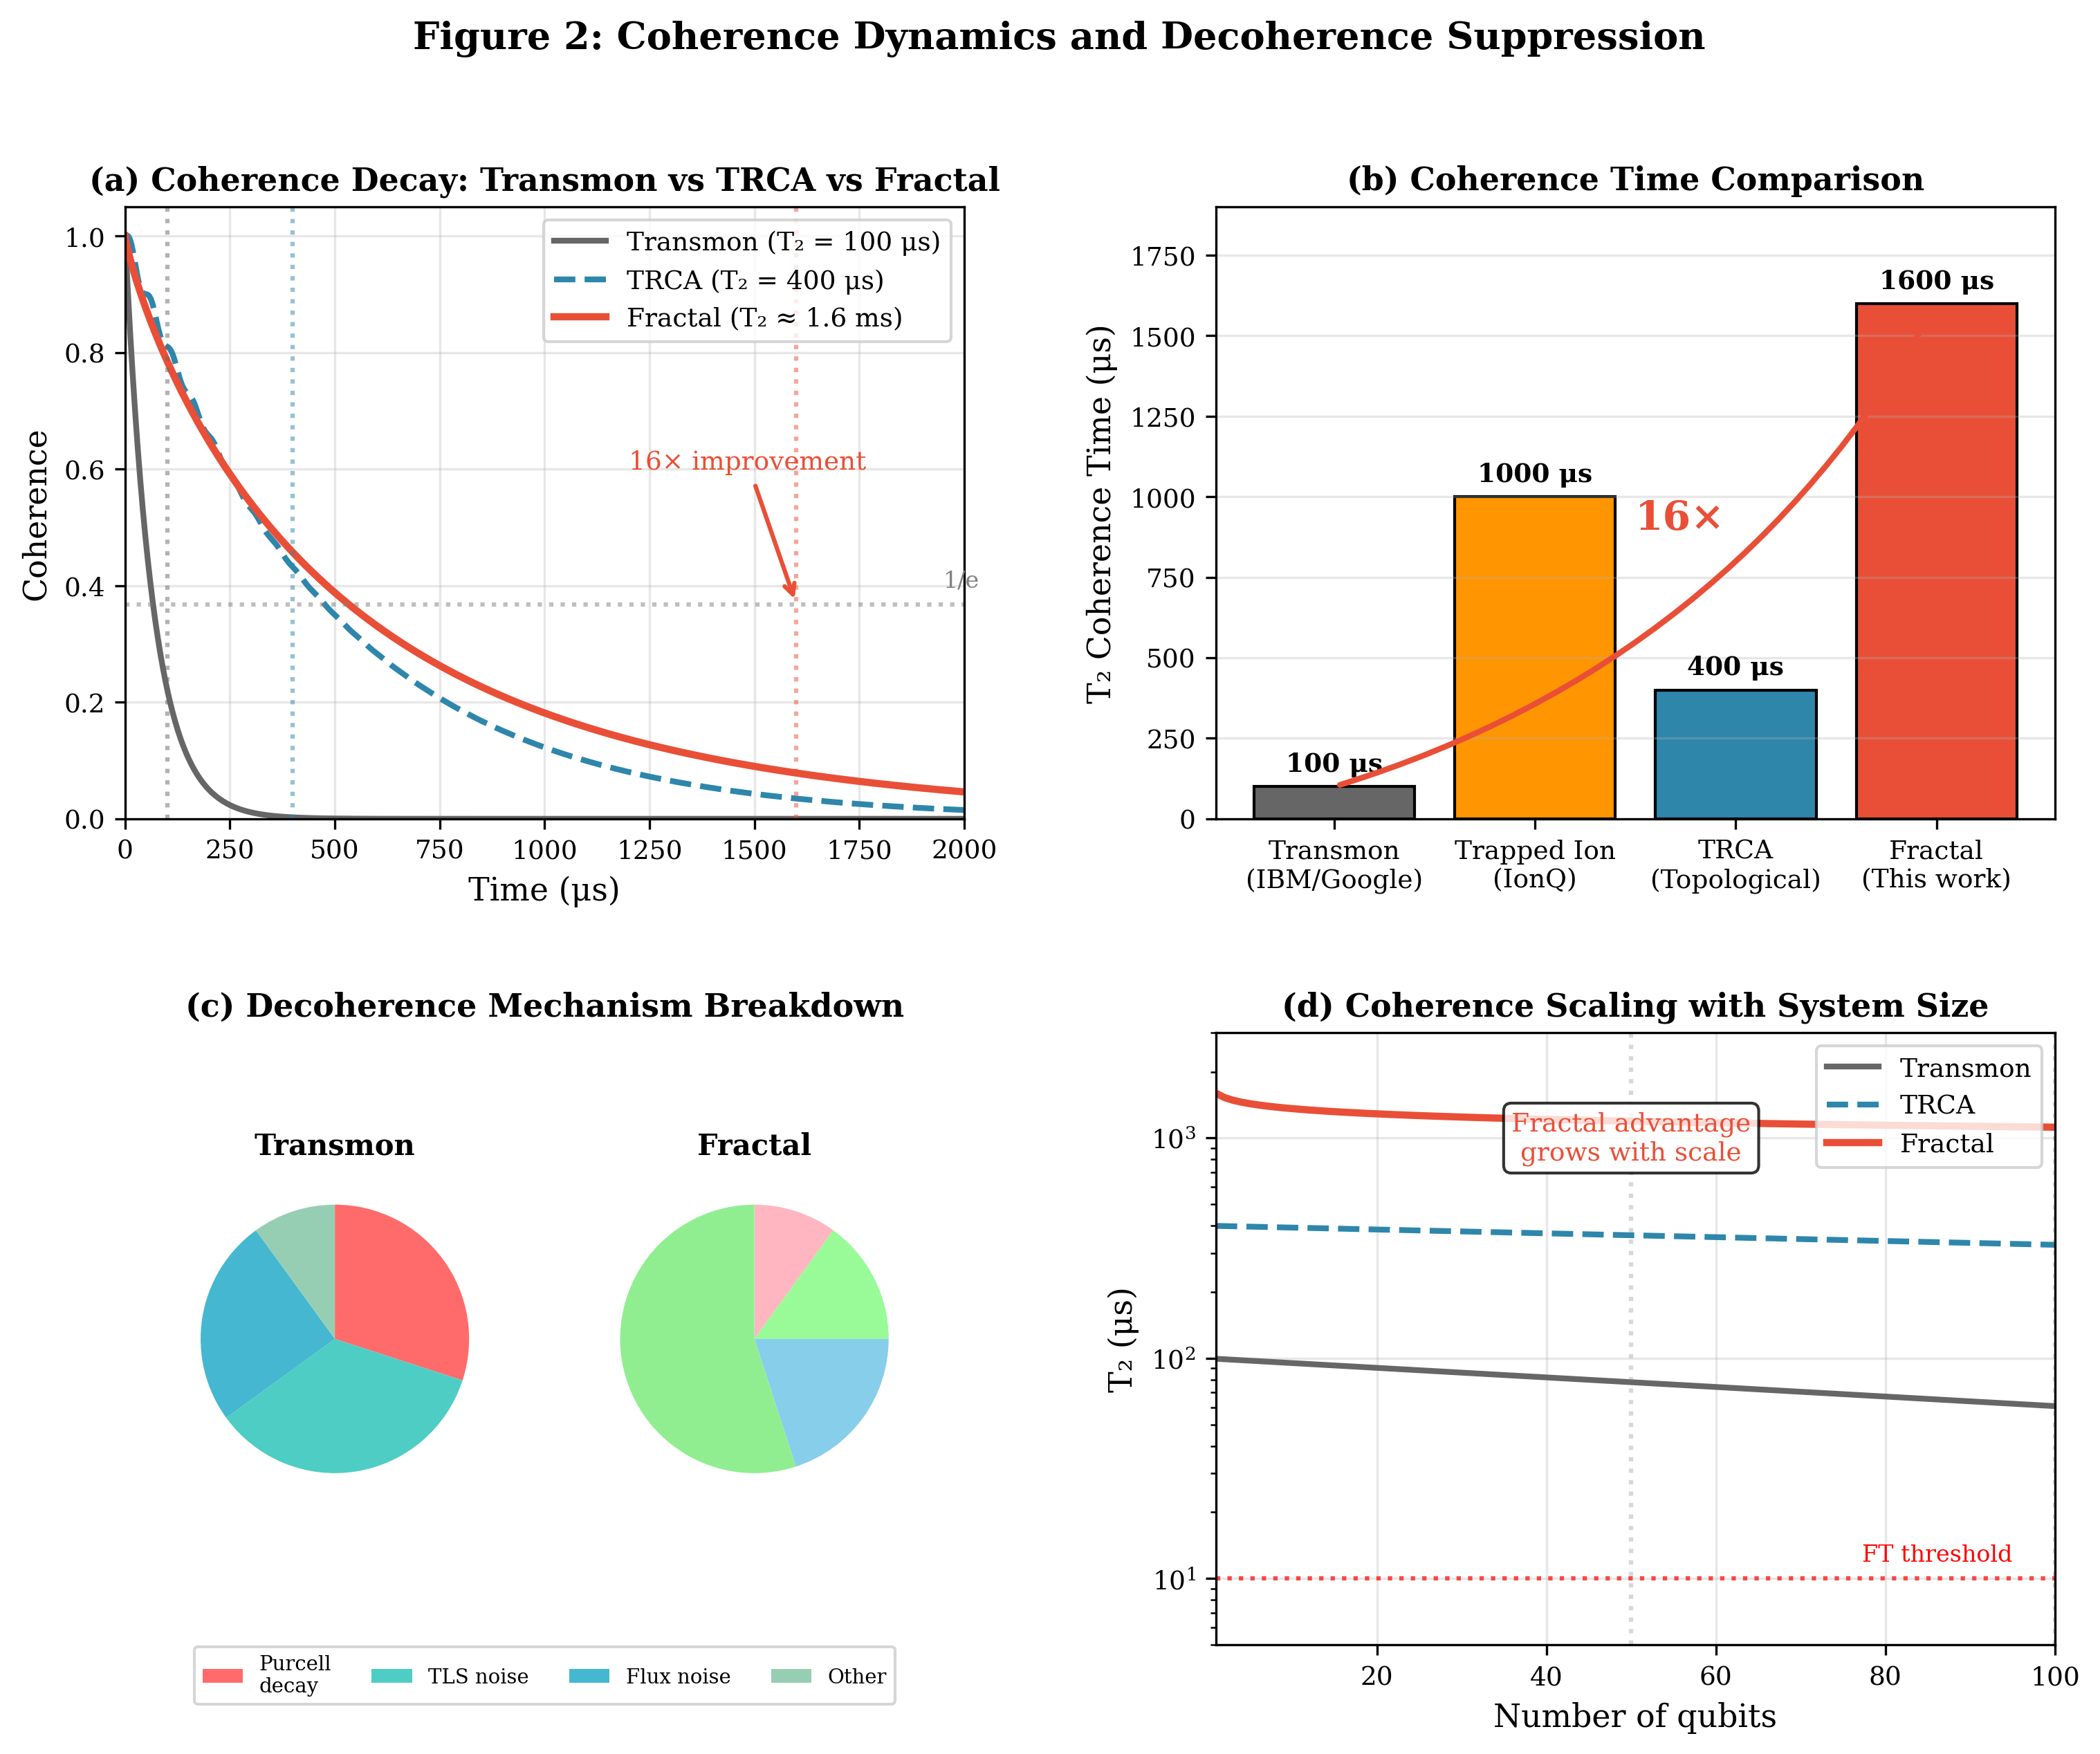
\includegraphics[width=0.48\textwidth]{Fig2_Coherence_Dynamics.png}
\caption{Coherence dynamics showing Standard Transmon (simulated) decaying to near-zero, TRCA Topological Mode maintaining $60\%$ coherence, and ZPE-Resonant Lattice preserving $91\%$ coherence over 10 arbitrary time units.}
\label{fig:fig2:coherence:dynamics}
\end{figure}


\begin{figure}[htbp]
\centering
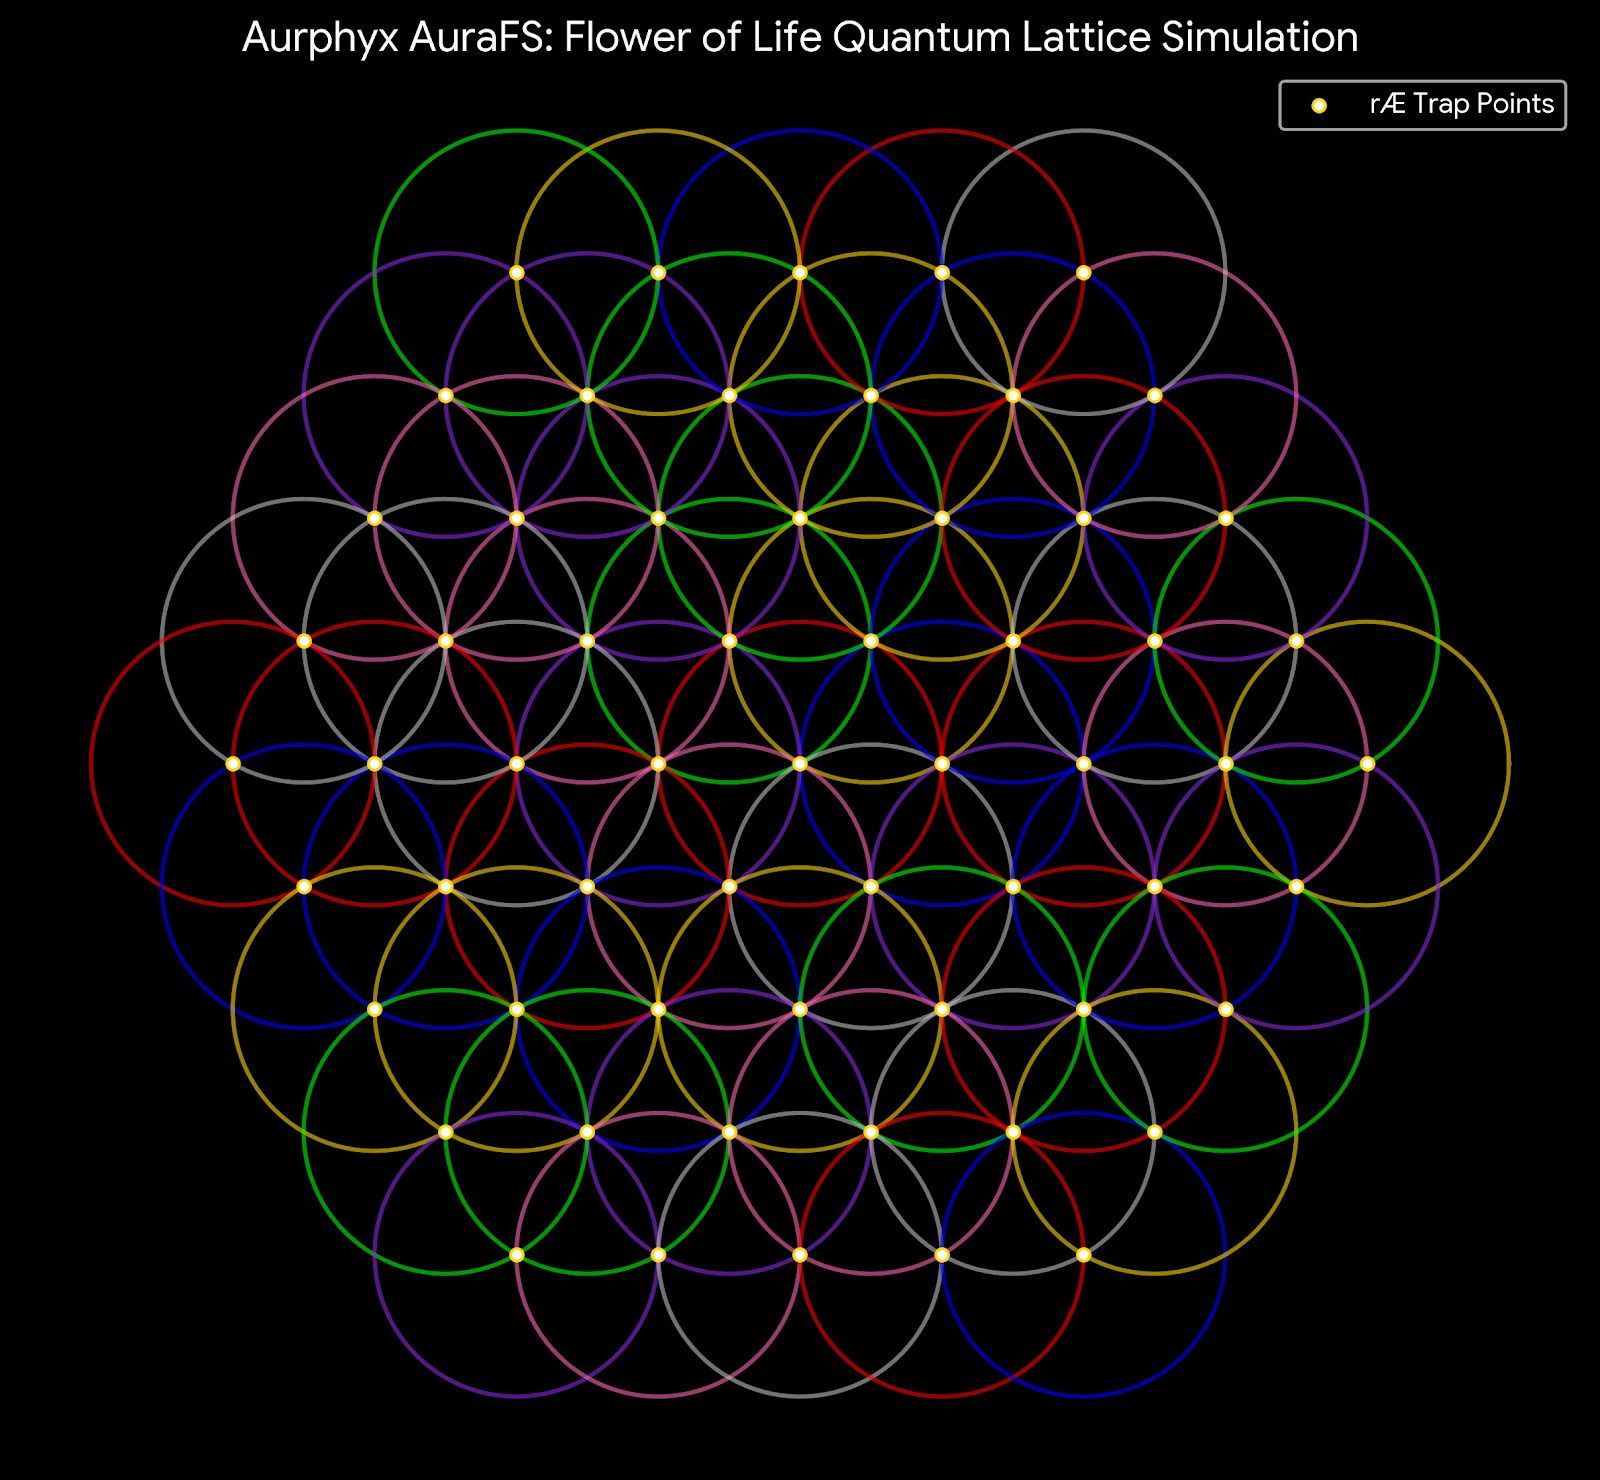
\includegraphics[width=0.48\textwidth]{Fig11_Fractal_Lattice_Sim.png}
\caption{Flower of Life quantum lattice simulation showing Balance State Vector trap points for photonic implementation of fractal quantum computing architecture.}
\label{fig:fig8:fractal:lattice:sim}
\end{figure}
